\noindentSection A (Questions 1--20, 1 mark each)
\begin{enumerate}[label=\thesubsection.\arabic*, ref=\thesubsection.\theenumi]
\item If the matrix $\vec{A} = \myvec{-p & q \\ r & p}$ is such that $\vec{A}^2 = \vec{I}$, then
\begin{enumerate}[label=(\Alph*)]
	\begin{multicols}{2}
	\item $1 + p^2 + qr = 0$
	\item $1 - p^2 - qr = 0$
	\item $1 - p^2 + qr = 0$
	\item $1 + p^2 - qr = 0$
	\end{multicols}
\end{enumerate}
\par\solution
\begin{align}
	\vec{A}^2 = \myvec{-p & q \\ r & p}\myvec{-p & q \\ r & p}
	= \myvec{p^2 + qr & 0 \\ 0 & p^2 + qr}
	= \brak{p^2+qr}\vec{I}
\end{align}
Hence $\vec{A}^2 = \vec{I}$ gives $p^2 + qr = 1$, i.e., $1 - p^2 - qr = 0$. Option (B).
The following code verifies this and the solutions of Problems~2, 4 and 5.
\begin{lstlisting}[frame=single, basicstyle=\rmfamily, escapeinside={(*@}{@*)}]
(*@\makebox[\dimexpr\linewidth-2\fboxsep-2\fboxrule\relax][c]{codes/Matrix.py}@*)
\end{lstlisting}

\item If $\vec{A}$ is a square matrix such that $\vec{A}^2 = \vec{A}$, then $\brak{\vec{A}-\vec{I}}^3 - \vec{A}$ is equal to
\begin{enumerate}[label=(\Alph*)]
	\begin{multicols}{4}
	\item $\vec{I}$
	\item $-\vec{I}$
	\item $\vec{A}$
	\item $\vec{A}^2$
	\end{multicols}
\end{enumerate}
\par\solution
Since $\vec{A}^2 = \vec{A}$,
\begin{align}
	\brak{\vec{A}-\vec{I}}^2 &= \vec{A}^2 - 2\vec{A} + \vec{I} = \vec{I} - \vec{A}
	\\
	\brak{\vec{A}-\vec{I}}^3 &= \brak{\vec{A}-\vec{I}}\brak{\vec{I}-\vec{A}} = -\brak{\vec{I}-\vec{A}}^2 
	= \vec{A} - \vec{I}
	\\
	\implies \brak{\vec{A}-\vec{I}}^3 - \vec{A} &= -\vec{I}
\end{align}
Option (B).

\item For the inverse trigonometric functions, which of the following principal value branches is not correctly defined?
\begin{enumerate}[label=(\Alph*)]
	\item $\tan^{-1}: \mathbb{R} \to \brak{-\frac{\pi}{2}, \frac{\pi}{2}}$
	\item $\sec^{-1}: \mathbb{R}-\brak{-1,1} \to \sbrak{0,\pi} - \cbrak{\frac{\pi}{2}}$
	\item $\cot^{-1}: \mathbb{R} \to \brak{0,\pi}$
	\item $\text{cosec}^{-1}: \mathbb{R}-\brak{-1,1} \to \sbrak{-\frac{\pi}{2}, \frac{\pi}{2}}$
\end{enumerate}
\par\solution
$\cosec x = \frac{1}{\sin x}$ is undefined at $\sin x = 0$, so $x = 0$ must be removed from the range. The correct branch is
\begin{align}
	\text{cosec}^{-1}: \mathbb{R}-\brak{-1,1} \to \sbrak{-\frac{\pi}{2}, \frac{\pi}{2}} - \cbrak{0}
\end{align}
The other three branches are the standard ones. Option (D).

\item Let $\vec{A} = \myvec{0 & -3 & 4 \\ 1 & 0 & 2}$ and $\vec{B} = \myvec{-3 & 0 & 1 \\ 2 & 4 & 0}$. If $\vec{A}+\vec{B}+\vec{C} = \vec{O}$, then the matrix $\vec{C}$ is
\begin{enumerate}[label=(\Alph*)]
	\begin{multicols}{2}
	\item $\myvec{-3 & -3 & 5 \\ 3 & 4 & 2}$
	\item $\myvec{3 & 3 & 5 \\ -3 & -4 & -2}$
	\item $\myvec{3 & 3 & -5 \\ -3 & -4 & -2}$
	\item $\myvec{-3 & -3 & -5 \\ 3 & 4 & 2}$
	\end{multicols}
\end{enumerate}
\par\solution
\begin{align}
	\vec{C} = -\brak{\vec{A}+\vec{B}} = -\myvec{-3 & -3 & 5 \\ 3 & 4 & 2}
	= \myvec{3 & 3 & -5 \\ -3 & -4 & -2}
\end{align}
Option (C).

\item If $\vec{A}$ is non-singular, which of the following is not true?
\begin{enumerate}[label=(\Alph*)]
	\begin{multicols}{2}
	\item $\text{adj}\,\vec{A}$ is singular
	\item $\brak{\text{adj}\,\vec{A}}^{-1} = \text{adj}\brak{\vec{A}^{-1}}$
	\item $\mydet{\vec{A}} \ne 0$
	\item $\vec{A}^{-1}$ exists
	\end{multicols}
\end{enumerate}
\par\solution
For a non-singular $\vec{A}$ of order $n$, from \eqref{eq:EE26BTECH11202-adj-det},
\begin{align}
	\mydet{\text{adj}\,\vec{A}} = \mydet{\vec{A}}^{n-1} \ne 0
\end{align}
so $\text{adj}\,\vec{A}$ is non-singular and statement (A) is false. Option (A).

\item If $f\brak{x} = \begin{cases} \dfrac{x^2-4x-5}{x+1}, & x \ne -1 \\ k, & x = -1 \end{cases}$
is continuous at $x = -1$, then the value of $k$ is
\begin{enumerate}[label=(\Alph*)]
	\begin{multicols}{2}
	\item Any real value
	\item $6$
	\item $-1$
	\item $-6$
	\end{multicols}
\end{enumerate}
\par\solution
Since $x^2-4x-5 = \brak{x-5}\brak{x+1}$, continuity requires
\begin{align}
	k = \lim_{x \to -1}\frac{\brak{x-5}\brak{x+1}}{x+1} = \lim_{x\to -1}\brak{x-5} = -6
\end{align}
Option (D).

\item If the area of $\triangle ABC$ with vertices $\vec{A} = \myvec{3 \\ 1}$, $\vec{B} = \myvec{-2 \\ 1}$ and $\vec{C} = \myvec{0 \\ k}$ is $5$ sq. units, then the values of $k$ are
\begin{enumerate}[label=(\Alph*)]
	\begin{multicols}{4}
	\item $3, 1$
	\item $-1, 3$
	\item $-1, 2$
	\item $0, 2$
	\end{multicols}
\end{enumerate}
\par\solution
\begin{align}
	\vec{B}-\vec{A} = \myvec{-5 \\ 0}, \quad \vec{C}-\vec{A} = \myvec{-3 \\ k-1}
\end{align}
From \eqref{eq:EE26BTECH11202-area},
\begin{align}
	\frac{1}{2}\abs{\mydet{-5 & -3 \\ 0 & k-1}} &= \frac{5}{2}\abs{k-1} = 5
	\\
	\implies k - 1 &= \pm 2 \implies k = 3 \text{ or } -1
\end{align}
Option (B). The code in Problem~25 verifies this.

\item The derivative of $\cos^{-1}\brak{\dfrac{\sin x + \cos x}{\sqrt{2}}}$, $-\dfrac{\pi}{4} < x < \dfrac{\pi}{4}$, with respect to $x$ is
\begin{enumerate}[label=(\Alph*)]
	\begin{multicols}{4}
	\item $-1$
	\item $1$
	\item $\frac{\pi}{4}$
	\item $-\frac{\pi}{4}$
	\end{multicols}
\end{enumerate}
\par\solution
\begin{align}
	\frac{\sin x + \cos x}{\sqrt{2}} = \myvec{\frac{1}{\sqrt{2}} & \frac{1}{\sqrt{2}}}\myvec{\sin x \\ \cos x}
	= \cos x\cos\frac{\pi}{4} + \sin x\sin\frac{\pi}{4} = \cos\brak{x-\frac{\pi}{4}}
\end{align}
For $-\frac{\pi}{4} < x < \frac{\pi}{4}$, we have $x - \frac{\pi}{4} \in \brak{-\frac{\pi}{2}, 0}$, so
\begin{align}
	\cos^{-1}\cos\brak{x-\frac{\pi}{4}} = \frac{\pi}{4} - x
	\implies \diff{}{x}\brak{\frac{\pi}{4}-x} = -1
\end{align}
Option (A).

\item The absolute minimum value of $f\brak{x} = \brak{x-2}^2 + 5$ in the interval $\sbrak{-3, 2}$ is
\begin{enumerate}[label=(\Alph*)]
	\begin{multicols}{4}
	\item $-3$
	\item $2$
	\item $5$
	\item $30$
	\end{multicols}
\end{enumerate}
\par\solution
\begin{align}
	f^{\prime}\brak{x} = 2\brak{x-2} < 0 \quad \text{for } x \in \left[-3, 2\right)
\end{align}
So $f$ is decreasing on $\sbrak{-3,2}$ and the minimum is at the right end,
$f\brak{2} = 5$. Option (C).

\item $\displaystyle\int \frac{1}{\sqrt{1+\cos 2x}}\,dx$ is equal to
\begin{enumerate}[label=(\Alph*)]
	\begin{multicols}{2}
	\item $\log\cos x + C$
	\item $\frac{1}{\sqrt{2}}\log\abs{\sec x + \tan x} + C$
	\item $\frac{1}{\sqrt{2}}\log\abs{\sec x - \tan x} + C$
	\item $\log\sin 2x + C$
	\end{multicols}
\end{enumerate}
\par\solution
Since $1 + \cos 2x = 2\cos^2 x$, taking $\cos x > 0$,
\begin{align}
	\int\frac{dx}{\sqrt{2}\cos x} = \frac{1}{\sqrt{2}}\int\sec x\,dx
	= \frac{1}{\sqrt{2}}\log\abs{\sec x + \tan x} + C
\end{align}
from \eqref{eq:EE26BTECH11202-int-sec}. Option (B).

\item The value of $\displaystyle\int_{-5}^{-1}\frac{1}{x}\,dx$ is equal to
\begin{enumerate}[label=(\Alph*)]
	\begin{multicols}{4}
	\item $-\log 5$
	\item $x^6$
	\item $\log\brak{-5}$
	\item $x^{-6}$
	\end{multicols}
\end{enumerate}
\par\solution
\begin{align}
	\int_{-5}^{-1}\frac{dx}{x} = \sbrak{\log\abs{x}}_{-5}^{-1} = \log 1 - \log 5 = -\log 5
\end{align}
Option (A).

\item An ant crawls on a sheet of paper along the line $y = 2x - 4$. The area of the surface bounded by the $y$-axis, the $x$-axis and $x = 1$ is
\begin{enumerate}[label=(\Alph*)]
	\begin{multicols}{4}
	\item $1$ sq. unit
	\item $3$ sq. units
	\item $2$ sq. units
	\item $4$ sq. units
	\end{multicols}
\end{enumerate}
\par\solution
For $0 \le x \le 1$ the line lies below the $x$-axis ($y$ goes from $-4$ to $-2$), so
\begin{align}
	\text{Area} = \int_0^1 \abs{2x-4}\,dx = \int_0^1\brak{4-2x}\,dx = \sbrak{4x - x^2}_0^1 = 3
\end{align}
This is a trapezium with parallel sides $4$ and $2$ and width $1$, i.e., $\frac{4+2}{2}\cdot 1 = 3$. Option (B).
The following code verifies and plots the graph

\begin{lstlisting}[frame=single, basicstyle=\rmfamily, escapeinside={(*@}{@*)}]
(*@\makebox[\dimexpr\linewidth-2\fboxsep-2\fboxrule\relax][c]{codes/Ant.py}@*)
\end{lstlisting}


\begin{figure}[H]
	\centering
	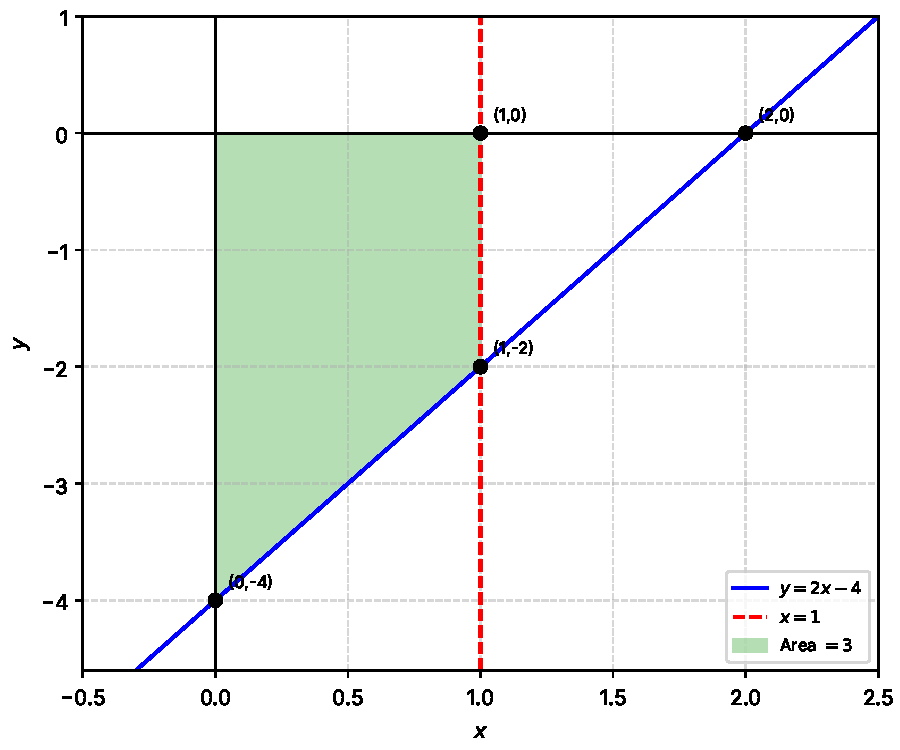
\includegraphics[width=0.6\linewidth]{figs/Ant.pdf}
	
\end{figure}




\item The general solution of the differential equation $\diff{y}{x} = e^{3x-y}$ is
\begin{enumerate}[label=(\Alph*)]
	\begin{multicols}{2}
	\item $3e^{y} = e^{3x} + C$
	\item $\log\brak{3x-y} = C$
	\item $e^{3x-y} = C$
	\item $-e^{y} + 3e^{3x} = C$
	\end{multicols}
\end{enumerate}
\par\solution
Separating the variables,
\begin{align}
	e^{y}\,dy = e^{3x}\,dx \implies e^{y} = \frac{e^{3x}}{3} + C^{\prime}
	\implies 3e^{y} = e^{3x} + C
\end{align}
Option (A).


\item If the position vector $\vec{p}$ of the point $\brak{24, n}$ satisfies $\norm{\vec{p}} = 25$, then $n$ is
\begin{enumerate}[label=(\Alph*)]
	\begin{multicols}{4}
	\item $\pm 49$
	\item $\pm 5$
	\item $\pm 1$
	\item $\pm 7$
	\end{multicols}
\end{enumerate}
\par\solution
\begin{align}
	\norm{\vec{p}}^2 = \myvec{24 & n}\myvec{24 \\ n} = 576 + n^2 = 625
	\implies n^2 = 49 \implies n = \pm 7
\end{align}
Option (D).

\item The vectors $\vec{a} = \myvec{3 \\ 2 \\ \lambda}$ and $\vec{b} = \myvec{2 \\ -4 \\ 5}$ represent the two strips of the Red Cross sign outside a doctor's clinic. The value of $\lambda$ is
\begin{enumerate}[label=(\Alph*)]
	\begin{multicols}{4}
	\item $1$
	\item $\frac{5}{2}$
	\item $\frac{2}{5}$
	\item $0$
	\end{multicols}
\end{enumerate}
\par\solution
The strips of the cross are perpendicular. From \eqref{eq:EE26BTECH11202-ortho},
\begin{align}
	\vec{a}^{\top}\vec{b} = 6 - 8 + 5\lambda = 0 \implies \lambda = \frac{2}{5}
\end{align}
Option (C).

\item If $3\pr{A} = \pr{B} = \dfrac{3}{5}$ and $\pr{A\vert B} = \dfrac{2}{3}$, then $\pr{A+B}$ is
\begin{enumerate}[label=(\Alph*)]
	\begin{multicols}{4}
	\item $\frac{3}{5}$
	\item $\frac{1}{5}$
	\item $\frac{2}{15}$
	\item $\frac{2}{5}$
	\end{multicols}
\end{enumerate}
\par\solution
Here $\pr{A} = \frac{1}{5}$ and $\pr{B} = \frac{3}{5}$. From \eqref{eq:EE26BTECH11202-cond},
\begin{align}
	\pr{AB} &= \pr{A\vert B}\pr{B} = \frac{2}{3}\cdot\frac{3}{5} = \frac{2}{5}
	\\
	\pr{A+B} &= \frac{1}{5} + \frac{3}{5} - \frac{2}{5} = \frac{2}{5}
\end{align}
Option (D). Note that the given data are not consistent, since $\pr{AB} > \pr{A}$; the answer follows from the formula as the paper intends.
The code in Problem~31 verifies this.



\vspace{2mm}
\noindentSection B (Questions 21--25, 2 marks each)
\begin{enumerate}[label=\thesubsection.\arabic*, ref=\thesubsection.\theenumi, start=21]
\item Evaluate $\sin\sbrak{\tan^{-1}\brak{\tan\frac{3\pi}{4}}}$.
\par\solution
$\tan\frac{3\pi}{4} = -1$ and the principal value of $\tan^{-1}$ lies in $\brak{-\frac{\pi}{2},\frac{\pi}{2}}$, so
\begin{align}
	\tan^{-1}\brak{-1} = -\frac{\pi}{4}
	\implies \sin\brak{-\frac{\pi}{4}} = -\frac{1}{\sqrt{2}}
\end{align}

\item 
(a) Differentiate $x^x$ with respect to $x\log x$.

OR

(b) If $y = P\cos ux + Q\sin ux$, show that $\diff{^2y}{x^2} + u^2y = 0$.
\par\solution
(a) Let $p = x^x$ and $q = x\log x$ for $x > 0$. Then $\log p = x\log x = q$, and from \eqref{eq:EE26BTECH11202-logdiff},
\begin{align}
	\diff{p}{x} &= x^x\brak{1+\log x}, \quad \diff{q}{x} = 1 + \log x
	\\
	\implies \diff{p}{q} &= \frac{dp/dx}{dq/dx} = x^x
\end{align}
(b) Differentiating twice,
\begin{align}
	\diff{y}{x} &= -Pu\sin ux + Qu\cos ux
	\\
	\diff{^2y}{x^2} &= -Pu^2\cos ux - Qu^2\sin ux = -u^2 y
	\\
	\implies \diff{^2y}{x^2} + u^2y &= 0
\end{align}
\textit{Remark:} this is the equation of a sinusoidal signal of angular frequency $u$, e.g., the voltage across an ideal LC tank.

\item Determine the values of $x$ for which $f\brak{x} = \dfrac{x-3}{x+1}$, $x \ne -1$, is an increasing function.
\par\solution
\begin{align}
	f^{\prime}\brak{x} = \frac{\brak{x+1} - \brak{x-3}}{\brak{x+1}^2} = \frac{4}{\brak{x+1}^2} > 0
	\quad \forall x \ne -1
\end{align}
Since $f^{\prime}\brak{x} > 0$, $f$ is increasing on $\brak{-\infty,-1}$ and on $\brak{-1,\infty}$, i.e., for all $x \in \mathbb{R}-\cbrak{-1}$.

\item 
(a) Three honey bees fly along the vectors $\vec{a} = \myvec{2 \\ -3 \\ 1}$, $\vec{b} = \myvec{0 \\ 4 \\ -2}$ and $\vec{c} = \myvec{3 \\ 0 \\ 2}$. Find $\lambda$ such that the path for $\vec{a}+\lambda\vec{b}$ is perpendicular to $\vec{c}$.

OR

(b) If $\vec{A}, \vec{B}, \vec{C}$ are non-collinear points with $\vec{AB} = \myvec{1 \\ 2 \\ -1}$ and $\vec{AC} = \myvec{2 \\ -3 \\ 0}$, find the area of $\triangle ABC$.
\par\solution
(a) From \eqref{eq:EE26BTECH11202-ortho},
\begin{align}
	\brak{\vec{a}+\lambda\vec{b}}^{\top}\vec{c} = \vec{a}^{\top}\vec{c} + \lambda\vec{b}^{\top}\vec{c} = 8 - 4\lambda = 0
	\implies \lambda = 2
\end{align}
(b) 
\begin{align}
	\vec{AB}\times\vec{AC} = \myvec{\brak{2}\brak{0}-\brak{-1}\brak{-3} \\ \brak{-1}\brak{2}-\brak{1}\brak{0} \\ \brak{1}\brak{-3}-\brak{2}\brak{2}}
	= \myvec{-3 \\ -2 \\ -7}
\end{align}
From \eqref{eq:EE26BTECH11202-area},
\begin{align}
	\text{Area} = \frac{1}{2}\sqrt{9+4+49} = \frac{\sqrt{62}}{2} \text{ sq. units}
\end{align}

\item Find the angle between the lines
\begin{align}
	\frac{x-2}{3} = \frac{y+5}{2} = \frac{1-z}{-6}, \qquad
	\frac{x-7}{1} = \frac{y}{2} = \frac{6-z}{-2}
\end{align}
\par\solution
Since $\frac{1-z}{-6} = \frac{z-1}{6}$ and $\frac{6-z}{-2} = \frac{z-6}{2}$, the direction vectors are
\begin{align}
	\vec{m}_1 = \myvec{3 \\ 2 \\ 6}, \quad \vec{m}_2 = \myvec{1 \\ 2 \\ 2},
	\quad \norm{\vec{m}_1} = 7, \; \norm{\vec{m}_2} = 3
\end{align}
From \eqref{eq:EE26BTECH11202-angle},
\begin{align}
	\cos\theta = \frac{3 + 4 + 12}{7 \cdot 3} = \frac{19}{21}
	\implies \theta = \cos^{-1}\brak{\frac{19}{21}} \approx 25.2\degree
\end{align}
The following code verifies this and Problems~7, 16, 17, 24, 30 and 35.
\begin{lstlisting}[frame=single, basicstyle=\rmfamily, escapeinside={(*@}{@*)}]
(*@\makebox[\dimexpr\linewidth-2\fboxsep-2\fboxrule\relax][c]{codes/Lines.py}@*)
\end{lstlisting}
\end{enumerate}

\vspace{2mm}
\noindentSection C (Questions 26--31, 3 marks each)
\begin{enumerate}[label=\thesubsection.\arabic*, ref=\thesubsection.\theenumi, start=26]
\item A spherical balloon loses its volume due to escape of air in such a way that the decrease of volume at any instant is proportional to its surface area. Show that the radius is decreasing at a constant rate.
\par\solution
Let $V = \frac{4}{3}\pi r^3$ and $S = 4\pi r^2$. For some constant $k > 0$,
\begin{align}
	\diff{V}{t} = -kS
	\implies 4\pi r^2\diff{r}{t} = -k\brak{4\pi r^2}
	\implies \diff{r}{t} = -k
\end{align}
which is a constant. Hence the radius decreases at a constant rate $k$.

\item 
(a) Find $\displaystyle\int\frac{x-\sin x}{1-\cos x}\,dx$.

OR

(b) Evaluate $\displaystyle\int_0^2\frac{1}{\sqrt{x^2+2x+3}}\,dx$.
\par\solution
(a) Using $1 - \cos x = 2\sin^2\frac{x}{2}$ and $\sin x = 2\sin\frac{x}{2}\cos\frac{x}{2}$,
\begin{align}
	\frac{x-\sin x}{1-\cos x} = \frac{x}{2}\text{cosec}^2\frac{x}{2} - \cot\frac{x}{2}
\end{align}
Integrating the first term by parts, with $u = x$ and $dv = \frac{1}{2}\text{cosec}^2\frac{x}{2}\,dx$,
\begin{align}
	\int\frac{x}{2}\text{cosec}^2\frac{x}{2}\,dx = -x\cot\frac{x}{2} + \int\cot\frac{x}{2}\,dx
\end{align}
The $\int\cot\frac{x}{2}\,dx$ terms cancel, so
\begin{align}
	\int\frac{x-\sin x}{1-\cos x}\,dx = -x\cot\frac{x}{2} + C
\end{align}
(b) Since $x^2+2x+3 = \brak{x+1}^2 + 2$, from \eqref{eq:EE26BTECH11202-int-root} with $a = \sqrt{2}$,
\begin{align}
	\int_0^2\frac{dx}{\sqrt{\brak{x+1}^2+2}}
	&= \sbrak{\log\abs{\brak{x+1}+\sqrt{x^2+2x+3}}}_0^2
	\\
	&= \log\brak{3+\sqrt{11}} - \log\brak{1+\sqrt{3}} = \log\frac{3+\sqrt{11}}{1+\sqrt{3}}
\end{align}
The following code verifies this and Problems~8, 10, 22, 23, 28 and 33.
\begin{lstlisting}[frame=single, basicstyle=\rmfamily, escapeinside={(*@}{@*)}]
(*@\makebox[\dimexpr\linewidth-2\fboxsep-2\fboxrule\relax][c]{codes/Calculus.py}@*)
\end{lstlisting}

\item Solve the differential equation $\brak{x + 2y^3}\,dy = y\,dx$.
\par\solution
Treating $x$ as a function of $y$,
\begin{align}
	\diff{x}{y} - \frac{1}{y}x = 2y^2
\end{align}
This is linear with integrating factor $e^{-\int dy/y} = \frac{1}{y}$. Hence
\begin{align}
	\diff{}{y}\brak{\frac{x}{y}} = 2y \implies \frac{x}{y} = y^2 + C
	\implies x = y^3 + Cy
\end{align}


\item 
(a) Three toys $A$, $B$ and $C$ are placed on a straight line. If their position vectors are $\myvec{55 \\ -2}$, $\myvec{5 \\ 8}$ and $\myvec{a \\ -52}$ respectively, find $a$.

OR

(b) If $\vec{a}, \vec{b}, \vec{c}$ are unit vectors, prove that $\norm{\vec{a}-\vec{b}}^2 + \norm{\vec{b}-\vec{c}}^2 + \norm{\vec{c}-\vec{a}}^2 \le 9$.
\par\solution
(a) From \eqref{eq:EE26BTECH11202-collinear},
\begin{align}
	\mydet{\vec{B}-\vec{A} & \vec{C}-\vec{A}} = \mydet{-50 & a-55 \\ 10 & -50}
	= 2500 - 10\brak{a-55} = 0 \implies a = 305
\end{align}
(b) Let $s = \vec{a}^{\top}\vec{b} + \vec{b}^{\top}\vec{c} + \vec{c}^{\top}\vec{a}$. Since the vectors are unit vectors, from \eqref{eq:EE26BTECH11202-norm-id},
\begin{align}
	\norm{\vec{a}-\vec{b}}^2 + \norm{\vec{b}-\vec{c}}^2 + \norm{\vec{c}-\vec{a}}^2 = 6 - 2s
\end{align}
But
\begin{align}
	0 \le \norm{\vec{a}+\vec{b}+\vec{c}}^2 = 3 + 2s \implies s \ge -\frac{3}{2}
\end{align}
Therefore
\begin{align}
	6 - 2s \le 6 + 3 = 9
\end{align}

\item 
(a) A die is rolled. For the events $A = \cbrak{1,2,5}$, $B = \cbrak{3,5}$, $C = \cbrak{2,3,4,5}$ find (i) $\pr{A\vert C}$ and $\pr{C\vert A}$, (ii) $\pr{AB\vert C}$ and $\pr{A+B\vert C}$.

OR

(b) A box contains cards numbered $1$ to $6$. Two cards are picked one by one with replacement. Let $A$ be the event that the sum of the numbers is $10$ and $B$ the event that the first card is not $4$. Find $\pr{AB}$ and state whether $A$ and $B$ are independent.
\par\solution
(a) Each outcome has probability $\frac{1}{6}$ and $AC = \cbrak{2,5}$, $AB = \cbrak{5}$, $\brak{A+B}C = \cbrak{2,3,5}$. From \eqref{eq:EE26BTECH11202-cond},
\begin{align}
	\pr{A\vert C} &= \frac{2/6}{4/6} = \frac{1}{2}, \quad
	\pr{C\vert A} = \frac{2/6}{3/6} = \frac{2}{3}
	\\
	\pr{AB\vert C} &= \frac{1/6}{4/6} = \frac{1}{4}, \quad
	\pr{A+B\vert C} = \frac{3/6}{4/6} = \frac{3}{4}
\end{align}
(b) There are $36$ equally likely outcomes. $A = \cbrak{\brak{4,6},\brak{5,5},\brak{6,4}}$ and $AB = \cbrak{\brak{5,5},\brak{6,4}}$, while $B$ has $5 \times 6 = 30$ outcomes. So
\begin{align}
	\pr{A} = \frac{1}{12}, \quad \pr{B} = \frac{5}{6}, \quad \pr{AB} = \frac{2}{36} = \frac{1}{18}
\end{align}
Now $\pr{A}\pr{B} = \frac{5}{72} \ne \frac{4}{72} = \pr{AB}$, so $A$ and $B$ are not independent.
The following code verifies this and Problems~18 and 37.
\begin{lstlisting}[frame=single, basicstyle=\rmfamily, escapeinside={(*@}{@*)}]
(*@\makebox[\dimexpr\linewidth-2\fboxsep-2\fboxrule\relax][c]{codes/Prob.py}@*)
\end{lstlisting}
\end{enumerate}

\vspace{2mm}
\noindentSection D (Questions 32--35, 5 marks each)
\begin{enumerate}[label=\thesubsection.\arabic*, ref=\thesubsection.\theenumi, start=32]
\item A man buys fruits. $4$ apples, $3$ oranges and $2$ bananas cost \rupee~$60$; $2$ apples, $4$ oranges and $6$ bananas cost \rupee~$90$; $6$ apples, $2$ oranges and $3$ bananas cost \rupee~$70$. Using the matrix method, find the cost of one fruit of each kind.
\par\solution
Let the prices of an apple, an orange and a banana be $x_1, x_2, x_3$. Then $\vec{A}\vec{x} = \vec{y}$ with
\begin{align}
	\vec{A} = \myvec{4 & 3 & 2 \\ 2 & 4 & 6 \\ 6 & 2 & 3}, \quad
	\vec{x} = \myvec{x_1 \\ x_2 \\ x_3}, \quad
	\vec{y} = \myvec{60 \\ 90 \\ 70}
\end{align}
Expanding along the first row,
\begin{align}
	\mydet{\vec{A}} = 4\brak{12-12} - 3\brak{6-36} + 2\brak{4-24} = 0 + 90 - 40 = 50 \ne 0
\end{align}
The cofactors are $C_{11}=0$, $C_{12}=30$, $C_{13}=-20$, $C_{21}=-5$, $C_{22}=0$, $C_{23}=10$, $C_{31}=10$, $C_{32}=-20$, $C_{33}=10$, so
\begin{align}
	\text{adj}\,\vec{A} = \myvec{0 & -5 & 10 \\ 30 & 0 & -20 \\ -20 & 10 & 10}
\end{align}
From \eqref{eq:EE26BTECH11202-adj} and \eqref{eq:EE26BTECH11202-linsys},
\begin{align}
	\vec{x} = \frac{1}{50}\myvec{0 & -5 & 10 \\ 30 & 0 & -20 \\ -20 & 10 & 10}\myvec{60 \\ 90 \\ 70}
	= \frac{1}{50}\myvec{250 \\ 400 \\ 400} = \myvec{5 \\ 8 \\ 8}
\end{align}
An apple costs \rupee~$5$, an orange \rupee~$8$ and a banana \rupee~$8$.
The following code verifies this.
\begin{lstlisting}[frame=single, basicstyle=\rmfamily, escapeinside={(*@}{@*)}]
(*@\makebox[\dimexpr\linewidth-2\fboxsep-2\fboxrule\relax][c]{codes/Fruits.py}@*)
\end{lstlisting}

\item 
(a) If $y\sqrt{x^2+1} = \log\brak{\sqrt{x^2+1}-x}$, show that $\brak{x^2+1}\diff{y}{x} + xy + 1 = 0$.

OR

(b) Find the derivative of $x^{\cot x} + \dfrac{2x^2-3}{2x^2-x+2}$ with respect to $x$.
\par\solution
(a) Let $s = \sqrt{x^2+1}$, so $\diff{s}{x} = \frac{x}{s}$. Differentiating $ys = \log\brak{s-x}$,
\begin{align}
	s\diff{y}{x} + \frac{xy}{s} = \frac{1}{s-x}\brak{\frac{x}{s} - 1} = \frac{1}{s-x}\cdot\frac{x-s}{s} = -\frac{1}{s}
\end{align}
Multiplying by $s$ and using $s^2 = x^2+1$,
\begin{align}
	\brak{x^2+1}\diff{y}{x} + xy + 1 = 0
\end{align}
(b) Let $u = x^{\cot x}$ and $v = \frac{2x^2-3}{2x^2-x+2}$. From \eqref{eq:EE26BTECH11202-logdiff},
\begin{align}
	\diff{u}{x} &= x^{\cot x}\diff{}{x}\brak{\cot x\log x} = x^{\cot x}\brak{\frac{\cot x}{x} - \text{cosec}^2 x\log x}
	\\
	\diff{v}{x} &= \frac{4x\brak{2x^2-x+2} - \brak{2x^2-3}\brak{4x-1}}{\brak{2x^2-x+2}^2}
	= \frac{-2x^2+20x-3}{\brak{2x^2-x+2}^2}
\end{align}
Hence
\begin{align}
	\diff{}{x}\brak{u+v} = x^{\cot x}\brak{\frac{\cot x}{x} - \text{cosec}^2 x\log x} + \frac{-2x^2+20x-3}{\brak{2x^2-x+2}^2}
\end{align}

\item Sketch the curve $\cbrak{\brak{x,y}: 100x^2 + 25y^2 = 2500}$ and find the area of the region enclosed by it using integration.
\par\solution
The curve is $\vec{x}^{\top}\vec{V}\vec{x} = c$ with
\begin{align}
	\vec{V} = \myvec{100 & 0 \\ 0 & 25}, \quad c = 2500
\end{align}
The eigenvalues of $\vec{V}$ are $100$ and $25$, so from \eqref{eq:EE26BTECH11202-ellipse} it is the ellipse
\begin{align}
	\frac{x^2}{25} + \frac{y^2}{100} = 1
\end{align}
with semi-axes $5$ along the $x$-axis and $10$ along the $y$-axis, symmetric about both axes (\figref{fig:EE26BTECH11202-2}). In the first quadrant $y = 2\sqrt{25-x^2}$, so by symmetry
\begin{align}
	\text{Area} &= 4\int_0^5 2\sqrt{25-x^2}\,dx = 8\sbrak{\frac{x}{2}\sqrt{25-x^2} + \frac{25}{2}\sin^{-1}\frac{x}{5}}_0^5
	\\
	&= 8\cdot\frac{25}{2}\cdot\frac{\pi}{2} = 50\pi \text{ sq. units}
\end{align}
which agrees with $\frac{\pi c}{\sqrt{\mydet{\vec{V}}}} = \frac{2500\pi}{50} = 50\pi$ from \eqref{eq:EE26BTECH11202-ellipse}.
The following code computes the area and generates \figref{fig:EE26BTECH11202-2}.
\begin{lstlisting}[frame=single, basicstyle=\rmfamily, escapeinside={(*@}{@*)}]
(*@\makebox[\dimexpr\linewidth-2\fboxsep-2\fboxrule\relax][c]{codes/Ellipse.py}@*)
\end{lstlisting}
\begin{figure}[H]
	\centering
	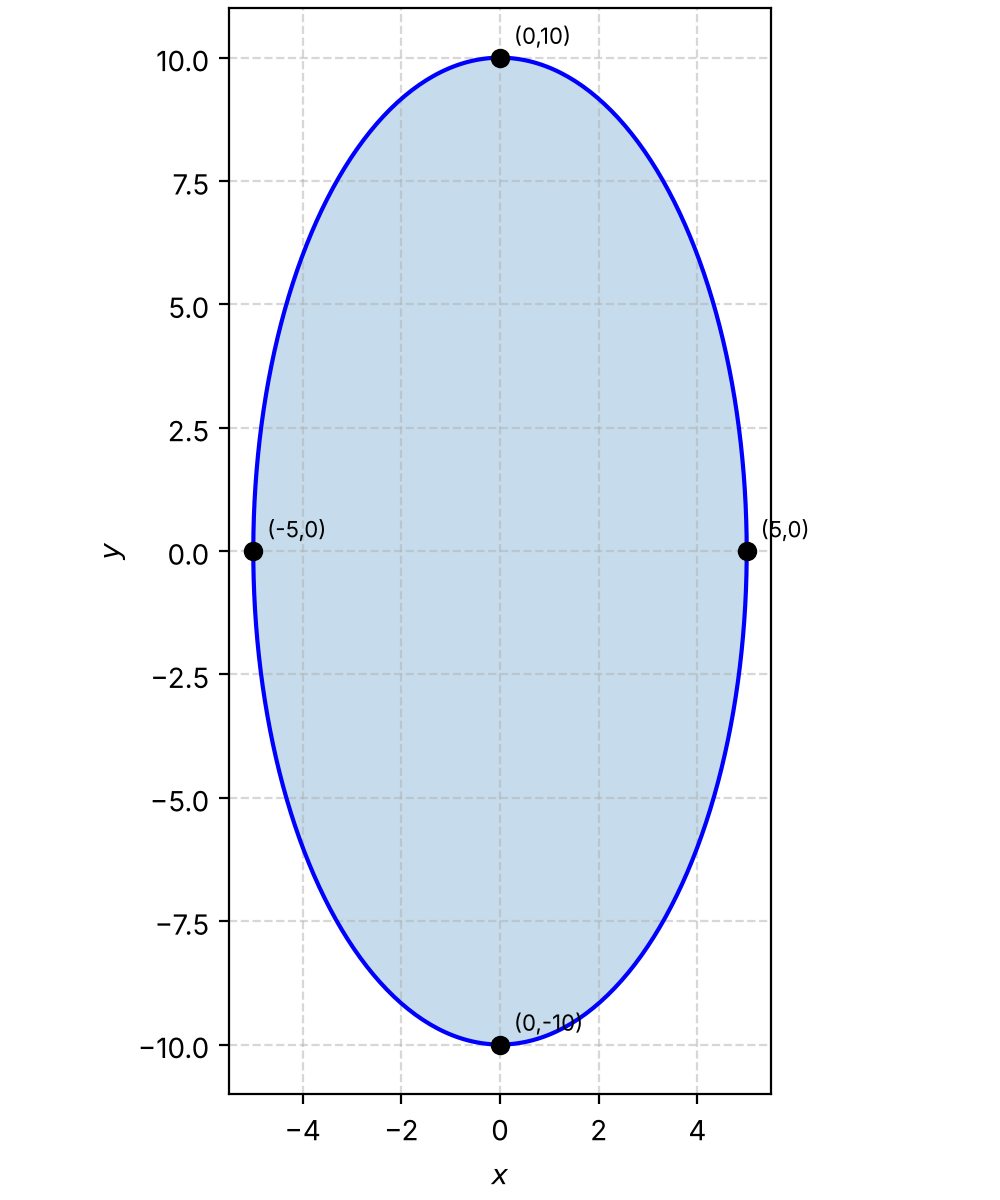
\includegraphics[width=0.5\linewidth]{figs/Ellipse.png}
	\caption{$100x^2+25y^2=2500$}
	\label{fig:EE26BTECH11202-2}
\end{figure}

\item 
(a) Find the foot of the perpendicular from the point $\vec{Q} = \myvec{0 \\ 2 \\ 3}$ on the line $\dfrac{-x-3}{-5} = \dfrac{1-y}{-2} = \dfrac{3z+12}{9}$ and hence the length of the perpendicular.

OR

(b) Find $p$ if the shortest distance between the lines $\vec{x} = \myvec{1 \\ 2 \\ 1} + \lambda\myvec{1 \\ -1 \\ 1}$ and $\vec{x} = \myvec{p \\ -1 \\ -1} + \mu\myvec{2 \\ 1 \\ 2}$ is $\dfrac{3}{\sqrt{2}}$ units.
\par\solution
(a) The line is $\frac{x+3}{5} = \frac{y-1}{2} = \frac{z+4}{3}$, i.e.,
\begin{align}
	\vec{x} = \vec{P}_0 + \lambda\vec{m}, \quad \vec{P}_0 = \myvec{-3 \\ 1 \\ -4}, \; \vec{m} = \myvec{5 \\ 2 \\ 3}
\end{align}
From \eqref{eq:EE26BTECH11202-foot},
\begin{align}
	\lambda_0 = \frac{\myvec{5 & 2 & 3}\myvec{3 \\ 1 \\ 7}}{\myvec{5 & 2 & 3}\myvec{5 \\ 2 \\ 3}} = \frac{38}{38} = 1
	\implies \vec{F} = \vec{P}_0 + \vec{m} = \myvec{2 \\ 3 \\ -1}
\end{align}
The length of the perpendicular is
\begin{align}
	\norm{\vec{F}-\vec{Q}} = \norm{\myvec{2 \\ 1 \\ -4}} = \sqrt{4+1+16} = \sqrt{21}
\end{align}
(b) 
\begin{align}
	\vec{m}_1\times\vec{m}_2 = \myvec{\brak{-1}\brak{2}-\brak{1}\brak{1} \\ \brak{1}\brak{2}-\brak{1}\brak{2} \\ \brak{1}\brak{1}-\brak{-1}\brak{2}} = \myvec{-3 \\ 0 \\ 3},
	\quad \norm{\vec{m}_1\times\vec{m}_2} = 3\sqrt{2}
\end{align}
With $\vec{A}_2-\vec{A}_1 = \myvec{p-1 \\ -3 \\ -2}$, from \eqref{eq:EE26BTECH11202-skew},
\begin{align}
	d = \frac{\abs{-3\brak{p-1} - 6}}{3\sqrt{2}} = \frac{\abs{p+1}}{\sqrt{2}} = \frac{3}{\sqrt{2}}
	\implies p + 1 = \pm 3 \implies p = 2 \text{ or } -4
\end{align}
\end{enumerate}

\vspace{2mm}
\noindentSection E (Questions 36--38, 4 marks each)
\begin{enumerate}[label=\thesubsection.\arabic*, ref=\thesubsection.\theenumi, start=36]


\item Case Study 2. Three vaccines $A_1, A_2, A_3$ were given to $25\%$, $35\%$ and $40\%$ of the population respectively. They protect against the infection with probabilities $60\%$, $55\%$ and $50\%$ respectively. Find the probability that
\begin{enumerate}[label=(\roman*)]
	\item a person taking vaccine $A_2$ gets infected. \hfill [1]
	\item a randomly chosen person is protected from the infection. \hfill [1]
	\item (a) the person was given vaccine $A_1$, given that the randomly chosen person is infected. \hfill [2]

	OR

	(b) the person was given vaccine $A_3$, given that the randomly chosen person is not infected. \hfill [2]
\end{enumerate}
\par\solution
Let $E$ be the event that the person is protected, and
\begin{align}
	\vec{p} = \myvec{0.25 \\ 0.35 \\ 0.40}, \quad \vec{q} = \myvec{0.60 \\ 0.55 \\ 0.50}
\end{align}
with $p_i = \pr{A_i}$ and $q_i = \pr{E\vert A_i}$.
\begin{enumerate}[label=(\roman*)]
	\item $\pr{E^{\prime}\vert A_2} = 1 - q_2 = 0.45 = \frac{9}{20}$.
	\item From \eqref{eq:EE26BTECH11202-total},
	\begin{align}
		\pr{E} = \vec{p}^{\top}\vec{q} = 0.15 + 0.1925 + 0.20 = 0.5425 = \frac{217}{400}
	\end{align}
	\item Here $\pr{E^{\prime}} = 1 - \frac{217}{400} = \frac{183}{400}$. From \eqref{eq:EE26BTECH11202-bayes},
	
	(a)
	\begin{align}
		\pr{A_1\vert E^{\prime}} = \frac{p_1\brak{1-q_1}}{\pr{E^{\prime}}} = \frac{0.25 \times 0.40}{0.4575} = \frac{40}{183} \approx 0.219
	\end{align}
	(b)
	\begin{align}
		\pr{A_3\vert E} = \frac{p_3 q_3}{\vec{p}^{\top}\vec{q}} = \frac{0.40\times 0.50}{0.5425} = \frac{80}{217} \approx 0.369
	\end{align}
\end{enumerate}

\item Case Study 3. A company produces cylindrical tumblers, open at the top, of fixed surface area. For a tumbler of volume $V$, height $h$ and base radius $r$ (\figref{fig:EE26BTECH11202-3}),
\begin{enumerate}[label=(\roman*)]
	\item differentiate $V$ with respect to $r$ when the surface area is constant. \hfill [2]
	\item if the volume is to be maximised, establish a relation between $h$ and $r$. \hfill [2]
\end{enumerate}
\begin{figure}[H]
	\centering
	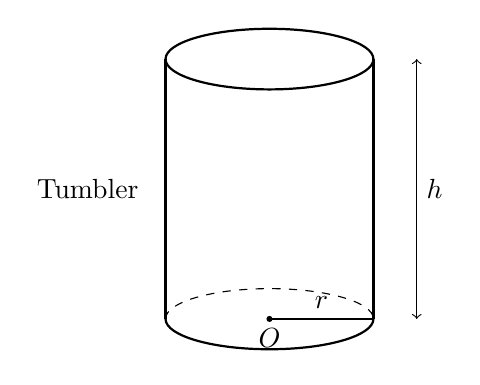
\begin{tikzpicture}[scale=1.1]
    \draw[thick] (-1.2, 0) -- (-1.2, 3);
    \draw[thick] (1.2, 0) -- (1.2, 3);
    \draw[thick] (0, 3) ellipse (1.2 and 0.35);
    \draw[thick] (-1.2, 0) arc (180:360:1.2 and 0.35);
    \draw[dashed] (-1.2, 0) arc (180:0:1.2 and 0.35);
    \fill (0, 0) circle (1pt) node[below] {$O$};
    \draw[thick] (0, 0) -- (1.2, 0) node[midway, above] {$r$};
    \draw[<->] (1.7, 0) -- (1.7, 3) node[midway, right] {$h$};
    \node[left] at (-1.4, 1.5) {Tumbler};
\end{tikzpicture}

	\caption{Open cylindrical tumbler}
	\label{fig:EE26BTECH11202-3}
\end{figure}
\par\solution
\begin{enumerate}[label=(\roman*)]
	\item The surface area (curved surface and base) is a constant $S$:
	\begin{align}
		S = \pi r^2 + 2\pi rh \implies h = \frac{S-\pi r^2}{2\pi r}
		\implies V = \pi r^2 h = \frac{Sr - \pi r^3}{2}
	\end{align}
	\begin{align}
		\diff{V}{r} = \frac{S - 3\pi r^2}{2} = \pi r\brak{h-r}
	\end{align}
	where the last step substitutes $S = \pi r^2 + 2\pi rh$.
	\item Setting $\diff{V}{r} = 0$ gives $h = r$ (equivalently $S = 3\pi r^2$). Also
	\begin{align}
		\diff{^2V}{r^2} = -3\pi r < 0
	\end{align}
	so $V$ is maximum when $\boxed{h = r}$. \figref{fig:EE26BTECH11202-4} shows $V$ against $r$ for $S = 3\pi$, with the maximum at $r = h = 1$.
	The following code verifies this and generates \figref{fig:EE26BTECH11202-4}.
\begin{lstlisting}[frame=single, basicstyle=\rmfamily, escapeinside={(*@}{@*)}]
(*@\makebox[\dimexpr\linewidth-2\fboxsep-2\fboxrule\relax][c]{codes/Tumbler.py}@*)
\end{lstlisting}
\begin{figure}[H]
	\centering
	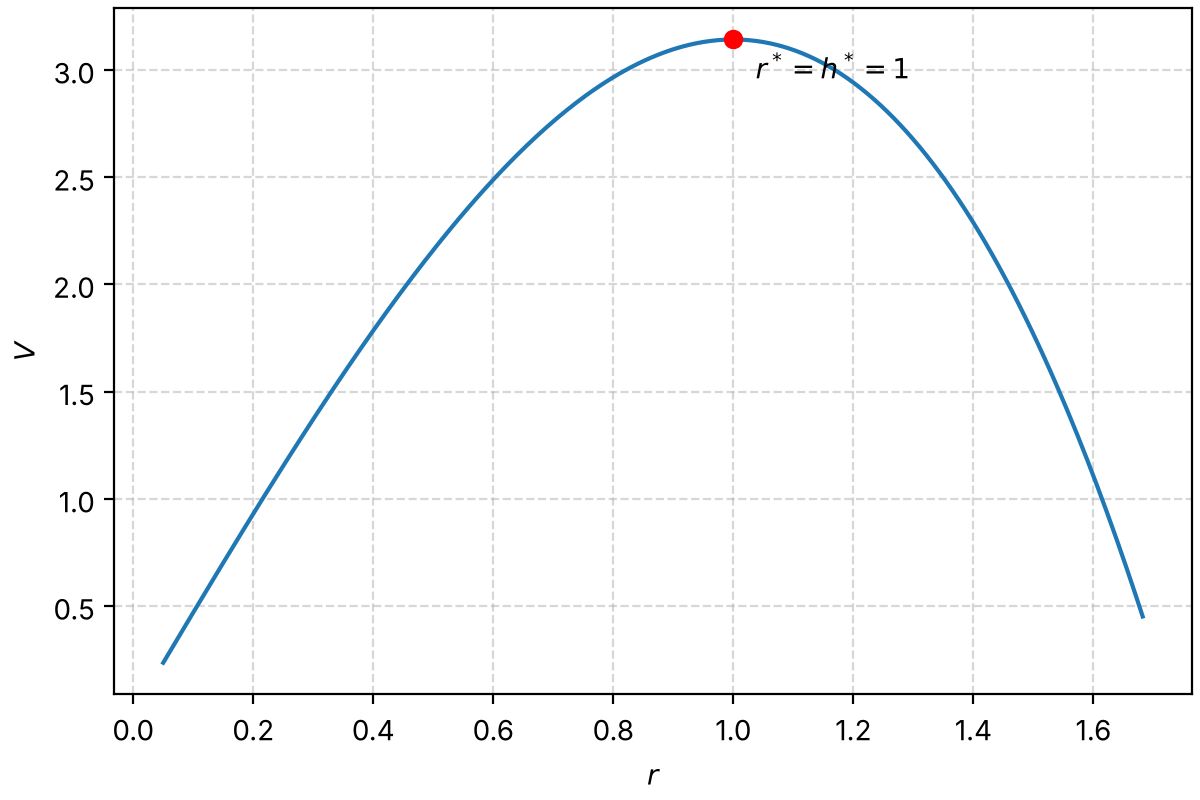
\includegraphics[width=0.6\linewidth]{figs/Tumbler_V.png}
	\caption{$V$ vs $r$ for $S = 3\pi$}
	\label{fig:EE26BTECH11202-4}
\end{figure}
\end{enumerate}
\end{enumerate}
